\documentclass[12pt]{exam}

\usepackage{amssymb,amsfonts,amsmath}
\usepackage[letterpaper,margin=1in]{geometry}
\usepackage{graphicx}
\usepackage[numbered]{matlab-prettifier}
\usepackage[]{mcode}
\usepackage{adjustbox}
\usepackage[T1]{fontenc}
\usepackage{mathtools}
\usepackage{color}
\usepackage{float}
\usepackage{bbold}

\DeclarePairedDelimiter{\abs}{\lvert}{\rvert}
\DeclarePairedDelimiter{\norm}{\lVert}{\rVert}

\renewcommand*{\vec}[1]{\boldsymbol{#1}}

\newcommand{\class}{Physics 306L}
\newcommand{\term}{Fall 2016}
\newcommand{\doctitle}{Lab Write-Up 8}

\parindent 0ex

\pagestyle{head}
\header{\bf \class}{\bf \doctitle\ - Page \thepage\ of \numpages}{\bf \term}
\headrule


\begin{document}

\begin{centering}
Week 8 - Analysis Active Filters - Op-Amps\\
\end{centering}
\begin{centering}
\textbf{General}\\
\end{centering}
\framebox{\parbox{\dimexpr\linewidth-2\fboxsep-2\fboxrule}{
\begin{centering}
\textbf{Lowpass Functions}\\
\end{centering}
$$Z_{\text{f}}= \frac{R_2}{R_1}$$\\
$$Z_{\text{in}} = 1+j\omega R_2C_1)$$\\
$$G(\omega) = -\frac{R2}{R1}\frac{1}{\j\omega R_2C_1 +1}$$\\
}}

\framebox{\parbox{\dimexpr\linewidth-2\fboxsep-2\fboxrule}{
\begin{centering}
\textbf{Bandpass Functions (Part 1 and Part 2)}\\
\end{centering}
$$Z_{\text{f}} = R_2 \parallel \frac{1}{j \omega C_2} $$\\ 
$$Z_{\text{in}} = R_1 + \frac{1}{j \omega C_1}$$ \\
$$G( \omega ) = -\frac{j \omega R_2 C_1}{(j \omega R_1 C_1+1)(j \omega C_2 R_2 +1)}$$
}}

\framebox{\parbox{\dimexpr\linewidth-2\fboxsep-2\fboxrule}{\begin{centering}
\textbf{Lowpass Filter}\\
\end{centering}
$R_{1}= 4506 \Omega $ , $R_{2}= 4552\Omega $, $C_{1}= 9.49  \times 10^{-9}$ F \\
Gain $= -1.01021 $ , Gain dB $=0.0882213 $ \\
Band $=3.68 \times 10^{3} Hz $ @ $-3$dB\\

\begin{centering}
\textbf{Functions}\\
\end{centering}
\begin{figure}[H]
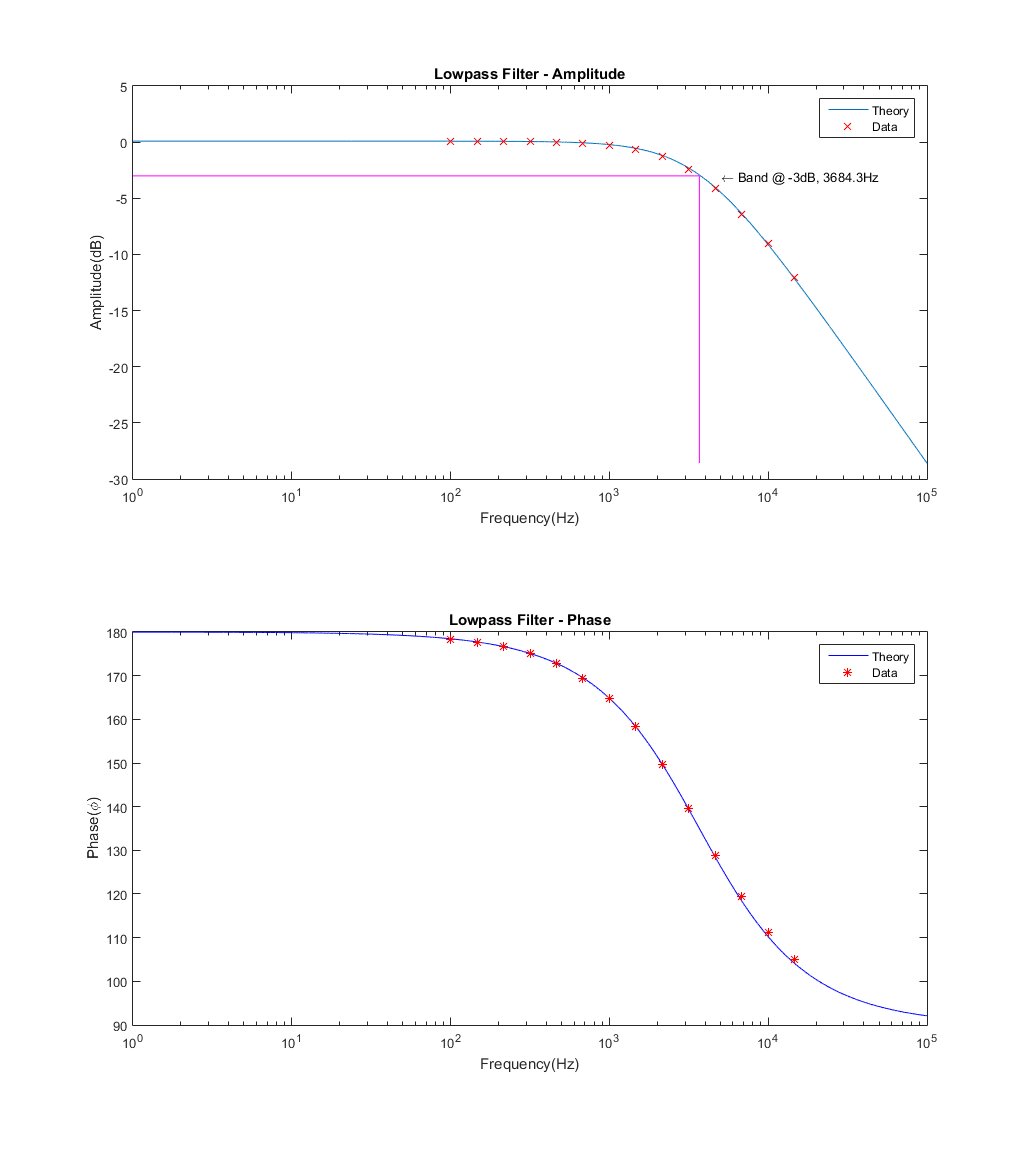
\includegraphics[width=\textwidth,keepaspectratio=true]{Lowpass.png}
\end{figure}
}}

\framebox{\parbox{\dimexpr\linewidth-2\fboxsep-2\fboxrule}{
\begin{centering}
\textbf{Bandpass Filter}\\
\end{centering}
$R_{1}= 465 \Omega $ , $R_{2}= 4552\Omega $, $C_{1}= 3.3  \times 10^{-7}$ F, $C_{2}   = 2.047\times  10^{-8}$ F \\
Gain $= 9.7892 $ , Gain dB $= 15.6934 $ \\
Band1 $= \frac{1}{465 \cdot 3.3 \times 10^{-07}} = 1.037\times 10^{3} $Hz\\
 Band 2 $= \frac{1}{4552 \Omega \cdot 2.047\times 10^{-08} F} = 1.71\times 10^{3}$Hz\\
\begin{figure}[H]
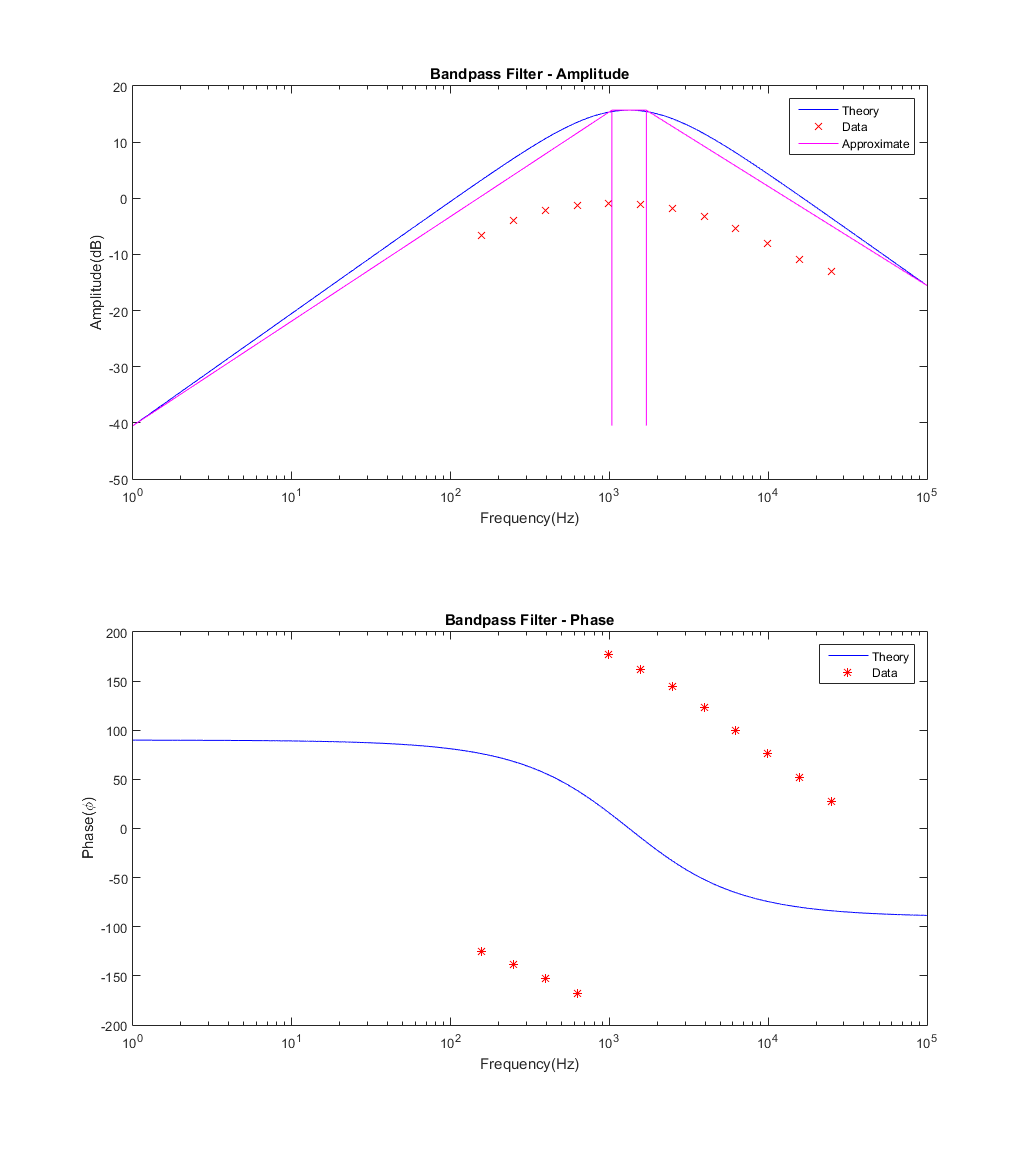
\includegraphics[width=\textwidth,keepaspectratio=true]{Bandpass.png}
\end{figure}
}}

\framebox{\parbox{\dimexpr\linewidth-2\fboxsep-2\fboxrule}{
\begin{centering}
\textbf{Bandpass Filter - Part 2}\\
\end{centering}
Chose $R_1 = R_2 = 10\Omega$\\
$C_{1}= 1.59 \times 10^{-8}$ F, $C_{2}   = 1.59\times  10^{-9}$ F \\
Gain $= 1 $ , Gain dB $= 0 $ \\
Band1 $= 10000 $Hz\\
Band2 $= 100000 $Hz\\
\begin{figure}[H]
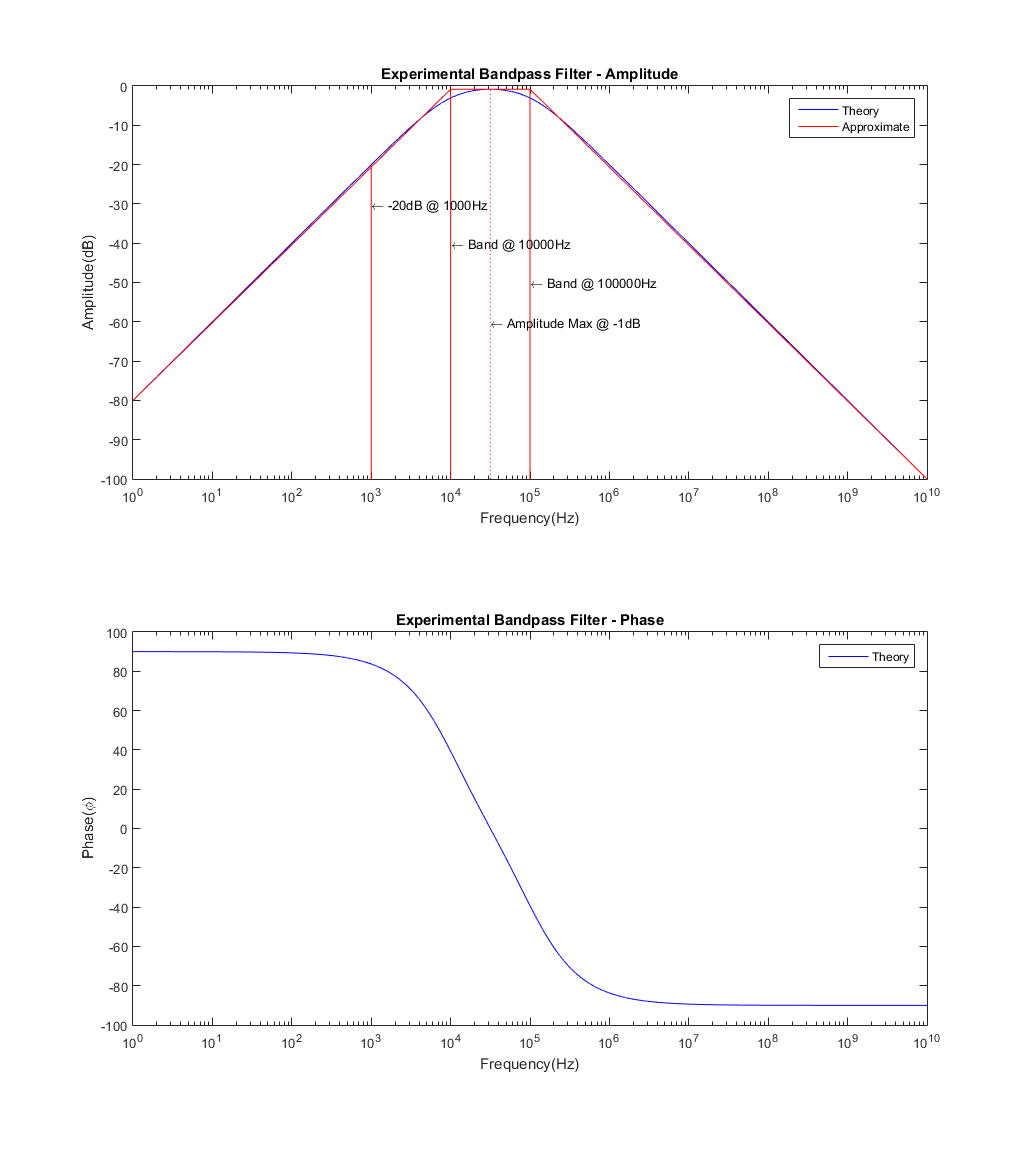
\includegraphics[width=\textwidth,keepaspectratio=true]{ExperimentalBandpass.png}
\end{figure}
}}



\end{document}
